\chapter{Realisierung}
% Dies ist das Hauptkapitel Ihrer Arbeit! Hier wird die Umsetzung der eigenen Ideen und Konzepte
% (Kapitel 3) anhand der gewählten Methoden (Kapitel 4) beschrieben, inkl. der dabei aufgetretenen
% Schwierigkeiten und Einschränkungen.
Die Realisierung lässt sich in drei Phasen unterteilen.

In der ersten Phase werden grundlegende Entscheidungen getroffen und die Basis der Arbeit implementiert.
Am Ende der ersten Phase existiert ein Prototyp, 
welcher die bei allen Komponenten des System die über minimalen Funktionen verfügt. (TODO verweis )

Wie im Kapitel Vorgehen beschrieben (TODO), folgen darauf zwei weitere Phasen,
in welche neue Anforderungen des Auftraggebers umgesetzt werden.


\section{Architekturentscheidung}

In dieser Arbeit wird keine Microservice Architektur im klassischen Sinne verwendet. (TODO "wie im xy erklärt")
Die einzelnen Komponenten werden zwar in separaten Container deployt (Abbildung: \ref{fig:smic-arch})
besitzen jedoch keine eigene Datenbank.
Das hat den Vorteil, dass weniger Overhead implementiert werden muss (mittels Message Queue)
und das Datenbankschema kann zentral in der Datastore Python library einmal implementiert
und dann in den verschiedenen Komponenten wiederverwendet werden.


\begin{figure}[h]
    \centering
    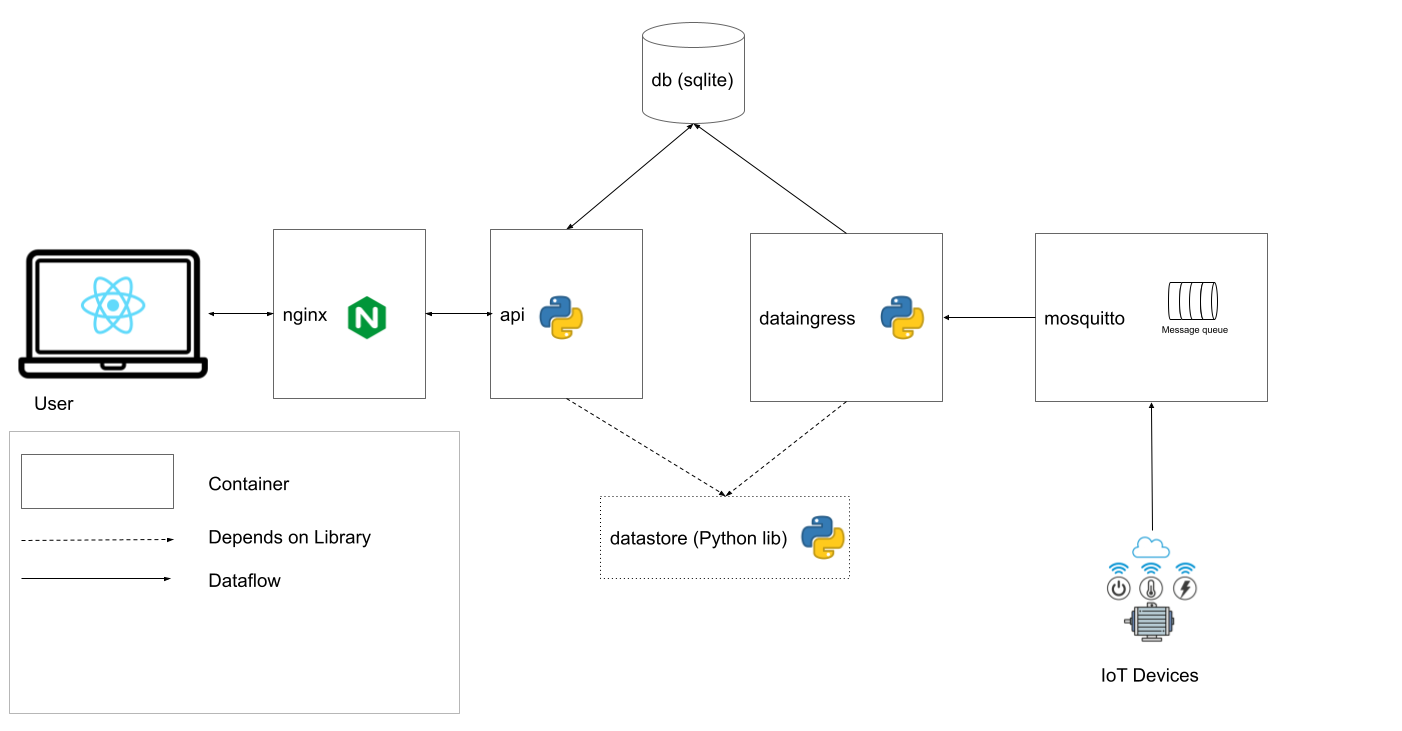
\includegraphics[width=1.0\textwidth]{gfx/smic-arch}
    \caption{
        Schamatische Darstellung der in diesem Projekt verwendeten Architektur
    }
    \label{fig:smic-arch}
\end{figure}

Die Abbildung \ref{fig:smic-arch} zeigt die in diesem Projekt verwendete
Architektur auf. Hier noch einige Informationen zu den einzelnen Komponenten:


\begin{itemize}
    \item \texttt{nginx}:
        Alle Anfragen des Endbenutzer werden über einen Nginx Server
        engegengenommen. Dieser liefert dann dem Benutzer die React WebApp
        oder leitet Anfragen an die \ac{API} weiter.

    \item \texttt{api}:
        Die \ac{API} verarbeitet Datenanfragen der React WebApp. Sie gibt
        beispielsweise die Stromzählerdaten eines Tages zurück.

    \item \texttt{datastore}:
        Der datastore ist eine Python library, die das Datenbankschema festlegt.
        Sowohl die \ac{API} als auch der dataingress greiffen auf die Datenbank zu
        und verwenden somit die datastore library.

    \item \texttt{dataingress}:
        Der dataingress arbeitet die von den \ac{IoT} geräten gesendeten
        Stromzählerdaten ab und speichert diese in die Datenbank.

    \item \texttt{mosquitto}:
        Mosquitto ist der in dieser Arbeit verwendete \ac{MQTT} Broker.
\end{itemize}

Ein weiterer grund für die Entscheidung einer geteilten Datenbank ist,
dass der \texttt{dataingress} keine Daten liest sondern diese nur von
der \ac{MQTT} Queue abarbeitet und in die Datenbank schreibt.

\section{Demo nach der ersten Phase}
Screenshot der ersten version
Rückmeldungen:
- grundsätzlich zufrieden
- Mobile nicht weiter zentral, Fokus auf Dashboard, Desktop

Neue Anforderungen:
Range/Zähler auswählen sowie typ der Daten
echte Daten automatisiert einspielen
THD und Power zusätzlich zu spannung

\section{Demon nach der zweiten Phase}
- Labeling:
Labels graphisch darstellen
Labels mittels UI hinzufügen
